Test Case~1a uses a set of five precomputed ground motion values to test the correct interpolation of the damage state exceedance probabilities of the discrete fragility function at intermediate intensity measure levels.

Table~\ref{tab:gmfs-diff-l1-5} lists the five ground motion values used in this test case.

\begin{table}[htbp]

\centering
\begin{tabular}{ c c c c c c c c c c }

\hline
\rowcolor{anti-flashwhite}
\bf{LS | PGA} & \bf{0.2g} & \bf{0.4g} & \bf{0.6g} & \bf{0.8g} & \bf{1.0g} & \bf{1.2g} & \bf{1.4g} & \bf{\dots} & \bf{5.0g} \\
\hline
\bf{ds1} & 0.000 & 0.152 & 0.846 & 0.993 & 1.000 & 1.000 & 1.000 & \dots & 1.000 \\
\bf{ds2} & 0.000 & 0.014 & 0.129 & 0.350 & 0.576 & 0.747 & 0.857 & \dots & 1.000 \\
\bf{ds3} & 0.000 & 0.008 & 0.085 & 0.196 & 0.325 & 0.450 & 0.561 & \dots & 0.993 \\
\bf{ds4} & 0.000 & 0.006 & 0.067 & 0.171 & 0.263 & 0.354 & 0.438 & \dots & 0.951 \\
\hline
\end{tabular}

\caption{Discrete fragility function with zero no damage limit}
\label{tab:ff-disc-tax1-zndl}
\end{table}

Table~\ref{tab:ff-disc-tax1-zndl} shows the set of ground motion intensity levels and corresponding probabilities of exceedance for the four damage states for the discrete fragility function used in this test case. The fragility model is shown in Figure~\ref{fig:ff-disc-tax1-zndl}.

\begin{figure}[htbp]
\centering
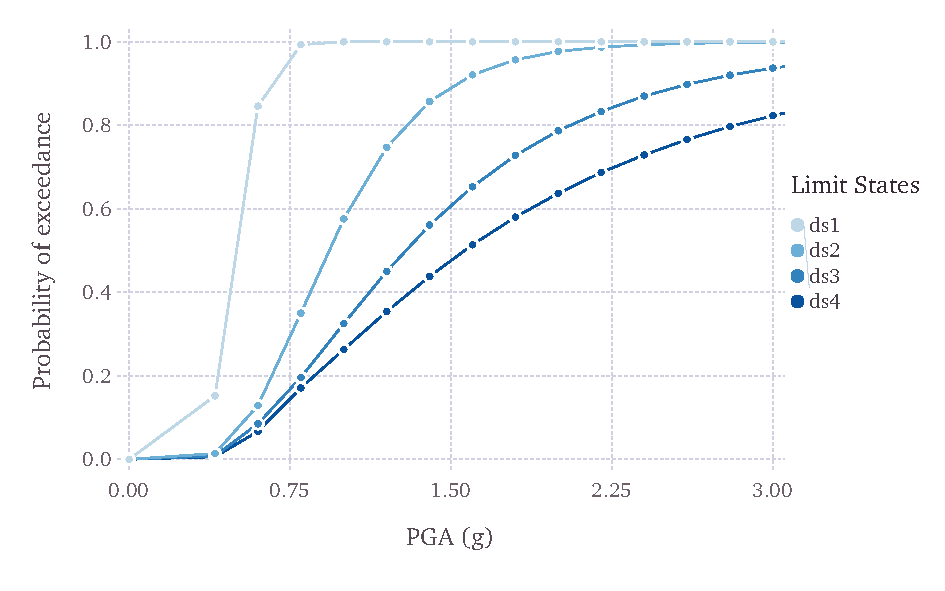
\includegraphics[width=12cm]{qareport/figures/fig-ff-disc-tax1-zndl}
\caption{Discrete fragility model with four damage states}
\label{fig:ff-disc-tax1-zndl}
\end{figure}

The ground motion values at the location of the single asset are $[1.3, 0.044, 0.52, 1.0, 1.2] g$. Consider the first value of $PGA = 1.3 g$. The discrete fragility function for this case provides damage state probabilities of exceedance at intensity measure levels $1.2 g$ and $1.4 g$, but none at $1.3 g$. The exceedance probabilities at $1.2 g$ and $1.4 g$ corresponding to the discrete damage states $[ds_1, ds_2, ds_3, ds_4]$ are $[1.000, 0.747, 0.450, 0.354]$ and $[1.000, 0.857, 0.561, 0.438]$ respectively.

The exceedance probabilities at $1.3 g$ are obtained by interpolating between these two sets of values. Linear interpolation gives exceedance probabilities of $[1.000, 0.802, 0.5055, 0.396]$ for $PGA = 1.3 g$. The probabilities of damage state occurrence are given by the pairwise differences of the exceedance probabilities as $[1.000 - 0.802, 0.802 - 0.5055, 0.5055 - 0.396, 0.396] = [0.198, 0.2965, 0.1095, 0.396]$. These four damage state probabilities sum up to one, indicating that the probability of observing no damage is zero.

Similar interpolation at the other four ground motion intensity levels gives the following sets of damage state probabilities:

\begin{itemize}
	\item GMF1: $[0.000, 0.198, 0.2965, 0.1095, 0.396]$
	\item GMF2: $[1.000, 0.000, 0.000, 0.000, 0.000]$
	\item GMF3: $[0.4316, 0.4854, 0.0288, 0.0116, 0.0426]$
	\item GMF4: $[0.000, 0.424, 0.251, 0.062, 0.263]$
	\item GMF5: $[0.000, 0.253, 0.297, 0.096, 0.354]$
\end{itemize}

The mean and standard deviation of the four damage state probabilities and also the probability of observing no damage is now calculated using the above set of probabilities collected from each of the five ground motion simulations.